\let\negmedspace\undefined
\let\negthickspace\undefined
\documentclass[journal]{IEEEtran}
\usepackage[a5paper, margin=10mm, onecolumn]{geometry}
%\usepackage{lmodern} % Ensure lmodern is loaded for pdflatex
\usepackage{tfrupee} % Include tfrupee package

\setlength{\headheight}{1cm} % Set the height of the header box
\setlength{\headsep}{0mm}     % Set the distance between the header box and the top of the text

\usepackage{gvv-book}
\usepackage{gvv}
\usepackage{cite}
\usepackage{amsmath,amssymb,amsfonts,amsthm}
\usepackage{algorithmic}
\usepackage{graphicx}
\usepackage{textcomp}
\usepackage{xcolor}
\usepackage{txfonts}
\usepackage{listings}
\usepackage{enumitem}
\usepackage{mathtools}
\usepackage{gensymb}
\usepackage{comment}
\usepackage[breaklinks=true]{hyperref}
\usepackage{tkz-euclide} 
\usepackage{listings}
% \usepackage{gvv}                                        
\def\inputGnumericTable{}                                 
\usepackage[latin1]{inputenc}                                
\usepackage{color}                                            
\usepackage{array}                                            
\usepackage{longtable}                                       
\usepackage{calc}                                             
\usepackage{multirow}                                         
\usepackage{hhline}                                           
\usepackage{ifthen}                                           
\usepackage{lscape}
\begin{document}

\bibliographystyle{IEEEtran}
\vspace{3cm}

\title{12.9.2.2}
\author{Balaji B - EE24BTECH11010}
% \maketitle
% \newpage
% \bigskip
{\let\newpage\relax\maketitle}

\renewcommand{\thefigure}{\theenumi}
\renewcommand{\thetable}{\theenumi}
\setlength{\intextsep}{10pt} % Space between text and floats


\numberwithin{equation}{enumi}
\numberwithin{figure}{enumi}
\renewcommand{\thetable}{\theenumi}

\textbf{Question:}\\
Consider the differential equation 
\begin{align}
    y^\prime - 2x - 2 = 0
\end{align}
Verify that
\begin{align}
    y = x^2 + 2x + C
\end{align}
is a solution for it.\\
\textbf{Theoretical Solution:}

The given differential equation is:
\begin{align}
    y^\prime - 2x - 2 = 0
\end{align}

Rearrange the terms to group all  $x$ and $y$ related terms:
\begin{align}
    y^\prime = 2x + 2
\end{align}

Now integrate both sides with respect to $x$:
\begin{align}
    \int y^\prime dx = \int \brak{2x + 2} dx
\end{align}

The left-hand side simplifies to  $y$, and the right-hand side is integrated term by term:
\begin{align}
    y = \int 2x dx + \int 2 dx \\
    y = x^2 + 2x + C
\end{align}

This matches the assumed solution:
\begin{align}
    y = x^2 + 2x + C
\end{align}
\textbf{Computational Solution: }\\ \\
The \textbf{ bilinear transform} is used to approximate the continuous derivative $y^{\prime}$ and reformulate the differential equation into a discrete time difference equation.\\ \\
Consider a first order differential equation of the form
\begin{align}
    y^\prime = f\brak{x,y}
\end{align}
The derivative $y^\prime$ in the equation is approximated using the bilinear transform. In the bilinear transform, the derivative is expressed in discrete form as: \\
\begin{align}
    y^\prime \approx \frac{y_{n+1} - y_n}{h}
\end{align}
Substituting this approximation into the general equation gives:
\begin{align}
    \frac{y_{n+1} - y_n}{h} = f\brak{x,y}
\end{align}
The Trapezoidal rule is applied to $f\brak{x,y}$ to approximate the value of $f\brak{x,y}$ over the interval $\sbrak{x_n,x_{n+1}}$.
\begin{align}
    f\brak{x,y} \approx \frac{1}{2} \sbrak{f\brak{x_n,y_n} + f\brak{x_{n+1},y_{n+1}}}
\end{align}
Substitute this into the discretized equation:
\begin{align}
    \frac{y_{n+1} - y_n}{h} = \frac{1}{2} \sbrak{f\brak{x_n,y_n} + f\brak{x_{n+1},y_{n+1}}}
\end{align}
Rearranging for $y_{n+1}$, we get 
\begin{align}
    y_{n+1} = y_{n} + \frac{h}{2} \sbrak{f\brak{x_n,y_n} + f\brak{x_{n+1},y_{n+1}}}
\end{align}
This is the general trapezoidal difference equation obtained using the bilinear transform.
Smaller the value of $h$ will give more precise plot. We obtain points to plot by repeatative iteration. \\
Substituting our $f\brak{x,y} = 2x+2$ in the above equation we get,
\begin{align}
    y_{n+1} = y_{n} + h\brak{x_{n} + x_{n+1}} + 2h 
\end{align}
The above equation is the required difference equation.\\ \\
Below is the comparison between the Theoretical plot and the simulated plot

\begin{figure}[h!]
   \centering
   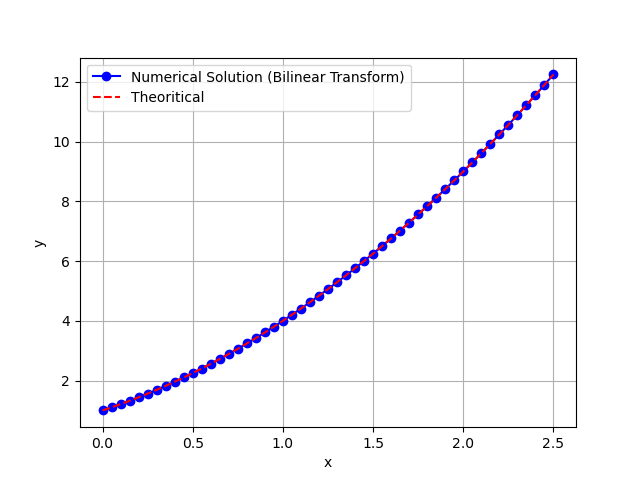
\includegraphics[width=1\columnwidth]{figs/fig.png}
   \caption{Computational vs Theoretical solution of $ y^\prime - 2x - 2 = 0$}
   \label{stemplot}
\end{figure}
\end{document}

